\section{Durchführung und Aufbau}
\label{sec:Durchführung}
Der Germaniumdetektor ist in diesem Versuch zur Messung von Gammaspektren bei radioaktiven Zerfällen von verschiedenen Isotopen benutzt worden. 
Dafür ist er, wie in Abbildung \ref{fig:germanium} dargestellt, in einem Bleigehäuse integriert worden. Der Detektor selbst ist von einer Aluminiumhülle umgeben, um niederenergetische Ereignisse herauszufiltern.
Zusätzlich wird er mit flüssigem Stickstoff gekühlt, um thermische Elektronenübergänge zu minimieren. Die Probe selbst wird in einem festen Abstand zum Detektor aufgehängt.
Der Germaniumdetektor ist, wie in Kapitel \ref{sec:Theorie} beschrieben, so aufgebaut, dass eine große Verarmungsschicht im Material entsteht. Dafür wird mit Lithium 
ein stark n-dotiertes Material auf der einen Seite und mit Gold ein p-dotiertes Material auf der anderen Seite des Germaniumkristalls aufgetragen und eine Spannung so angelegt, dass die Ladungen an den dotierten Schichten 
abfließen. Dafür ist eine Spannungsquelle an den Detektor angeschlossen. Die Detektion erfolgt dann über eine, wie in Kapitel \ref{ssec:Signalverarbeitung} beschriebene, Elektronik. Die Signale werden gemäß ihrer Stärke 
am Ende in einem Multichannelanalyzer (MCA) gespeichert und von einem Computer ausgelesen. 
\begin{figure}[H]
    \centering
    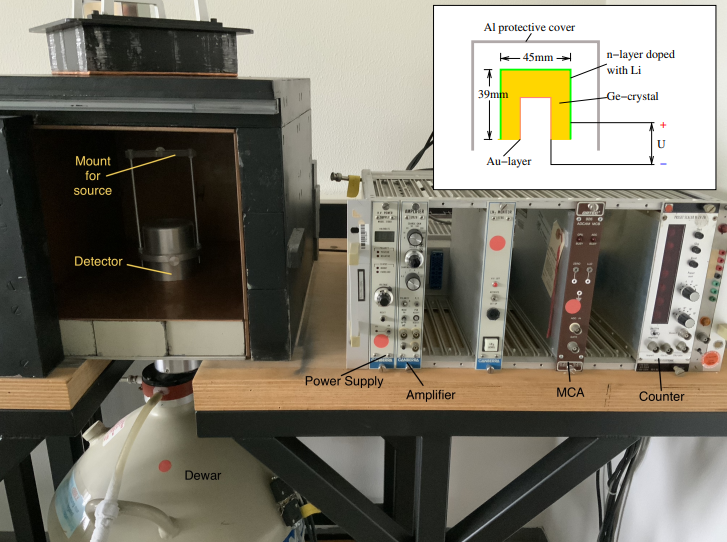
\includegraphics[scale=0.8]{illustration/Aufbau.png}
    \caption{Aufbau einer Gammaspektroskopie-Messschaltung und Aufbau des verwendeten Germaniumdetektors \cite{V18}}
    \label{fig:germanium}
\end{figure}
\noindent Mit dieser Apparatur sind nun 4 Proben gemessen worden: $^{152}$Eu, $^{137}$Cs, $^{133}$Ba und eine unbekannte Probe.
Die Proben wurden dafür nacheinander im Bleigehäuse platziert. Die Messung läuft dann vollständig automatisiert ab und muss nur am Computer gestartet werden. 
Für ein aussagekräftiges Spektrum wurden die Proben jeweils für 1 Stunde gemessen.
Zusätzlich wurde eine Untergrundmessung für einen Tag durchgeführt, in der keine Probe im Bleigehäuse war.
